\documentclass[
  stu,
  floatsintext,
  longtable,
  a4paper,
  nolmodern,
  notxfonts,
  notimes,
  colorlinks=true,linkcolor=blue,citecolor=blue,urlcolor=blue]{apa7}

\usepackage{amsmath}
\usepackage{amssymb}




\RequirePackage{longtable}
\RequirePackage{threeparttablex}

\makeatletter
\renewcommand{\paragraph}{\@startsection{paragraph}{4}{\parindent}%
	{0\baselineskip \@plus 0.2ex \@minus 0.2ex}%
	{-.5em}%
	{\normalfont\normalsize\bfseries\typesectitle}}

\renewcommand{\subparagraph}[1]{\@startsection{subparagraph}{5}{0.5em}%
	{0\baselineskip \@plus 0.2ex \@minus 0.2ex}%
	{-\z@\relax}%
	{\normalfont\normalsize\bfseries\itshape\hspace{\parindent}{#1}\textit{\addperi}}{\relax}}
\makeatother




\usepackage{longtable, booktabs, multirow, multicol, colortbl, hhline, caption, array, float, xpatch}
\usepackage{subcaption}


\renewcommand\thesubfigure{\Alph{subfigure}}
\setcounter{topnumber}{2}
\setcounter{bottomnumber}{2}
\setcounter{totalnumber}{4}
\renewcommand{\topfraction}{0.85}
\renewcommand{\bottomfraction}{0.85}
\renewcommand{\textfraction}{0.15}
\renewcommand{\floatpagefraction}{0.7}

\usepackage{tcolorbox}
\tcbuselibrary{listings,theorems, breakable, skins}
\usepackage{fontawesome5}

\definecolor{quarto-callout-color}{HTML}{909090}
\definecolor{quarto-callout-note-color}{HTML}{0758E5}
\definecolor{quarto-callout-important-color}{HTML}{CC1914}
\definecolor{quarto-callout-warning-color}{HTML}{EB9113}
\definecolor{quarto-callout-tip-color}{HTML}{00A047}
\definecolor{quarto-callout-caution-color}{HTML}{FC5300}
\definecolor{quarto-callout-color-frame}{HTML}{ACACAC}
\definecolor{quarto-callout-note-color-frame}{HTML}{4582EC}
\definecolor{quarto-callout-important-color-frame}{HTML}{D9534F}
\definecolor{quarto-callout-warning-color-frame}{HTML}{F0AD4E}
\definecolor{quarto-callout-tip-color-frame}{HTML}{02B875}
\definecolor{quarto-callout-caution-color-frame}{HTML}{FD7E14}

%\newlength\Oldarrayrulewidth
%\newlength\Oldtabcolsep


\usepackage{hyperref}



\usepackage{color}
\usepackage{fancyvrb}
\newcommand{\VerbBar}{|}
\newcommand{\VERB}{\Verb[commandchars=\\\{\}]}
\DefineVerbatimEnvironment{Highlighting}{Verbatim}{commandchars=\\\{\}}
% Add ',fontsize=\small' for more characters per line
\usepackage{framed}
\definecolor{shadecolor}{RGB}{241,243,245}
\newenvironment{Shaded}{\begin{snugshade}}{\end{snugshade}}
\newcommand{\AlertTok}[1]{\textcolor[rgb]{0.68,0.00,0.00}{#1}}
\newcommand{\AnnotationTok}[1]{\textcolor[rgb]{0.37,0.37,0.37}{#1}}
\newcommand{\AttributeTok}[1]{\textcolor[rgb]{0.40,0.45,0.13}{#1}}
\newcommand{\BaseNTok}[1]{\textcolor[rgb]{0.68,0.00,0.00}{#1}}
\newcommand{\BuiltInTok}[1]{\textcolor[rgb]{0.00,0.23,0.31}{#1}}
\newcommand{\CharTok}[1]{\textcolor[rgb]{0.13,0.47,0.30}{#1}}
\newcommand{\CommentTok}[1]{\textcolor[rgb]{0.37,0.37,0.37}{#1}}
\newcommand{\CommentVarTok}[1]{\textcolor[rgb]{0.37,0.37,0.37}{\textit{#1}}}
\newcommand{\ConstantTok}[1]{\textcolor[rgb]{0.56,0.35,0.01}{#1}}
\newcommand{\ControlFlowTok}[1]{\textcolor[rgb]{0.00,0.23,0.31}{\textbf{#1}}}
\newcommand{\DataTypeTok}[1]{\textcolor[rgb]{0.68,0.00,0.00}{#1}}
\newcommand{\DecValTok}[1]{\textcolor[rgb]{0.68,0.00,0.00}{#1}}
\newcommand{\DocumentationTok}[1]{\textcolor[rgb]{0.37,0.37,0.37}{\textit{#1}}}
\newcommand{\ErrorTok}[1]{\textcolor[rgb]{0.68,0.00,0.00}{#1}}
\newcommand{\ExtensionTok}[1]{\textcolor[rgb]{0.00,0.23,0.31}{#1}}
\newcommand{\FloatTok}[1]{\textcolor[rgb]{0.68,0.00,0.00}{#1}}
\newcommand{\FunctionTok}[1]{\textcolor[rgb]{0.28,0.35,0.67}{#1}}
\newcommand{\ImportTok}[1]{\textcolor[rgb]{0.00,0.46,0.62}{#1}}
\newcommand{\InformationTok}[1]{\textcolor[rgb]{0.37,0.37,0.37}{#1}}
\newcommand{\KeywordTok}[1]{\textcolor[rgb]{0.00,0.23,0.31}{\textbf{#1}}}
\newcommand{\NormalTok}[1]{\textcolor[rgb]{0.00,0.23,0.31}{#1}}
\newcommand{\OperatorTok}[1]{\textcolor[rgb]{0.37,0.37,0.37}{#1}}
\newcommand{\OtherTok}[1]{\textcolor[rgb]{0.00,0.23,0.31}{#1}}
\newcommand{\PreprocessorTok}[1]{\textcolor[rgb]{0.68,0.00,0.00}{#1}}
\newcommand{\RegionMarkerTok}[1]{\textcolor[rgb]{0.00,0.23,0.31}{#1}}
\newcommand{\SpecialCharTok}[1]{\textcolor[rgb]{0.37,0.37,0.37}{#1}}
\newcommand{\SpecialStringTok}[1]{\textcolor[rgb]{0.13,0.47,0.30}{#1}}
\newcommand{\StringTok}[1]{\textcolor[rgb]{0.13,0.47,0.30}{#1}}
\newcommand{\VariableTok}[1]{\textcolor[rgb]{0.07,0.07,0.07}{#1}}
\newcommand{\VerbatimStringTok}[1]{\textcolor[rgb]{0.13,0.47,0.30}{#1}}
\newcommand{\WarningTok}[1]{\textcolor[rgb]{0.37,0.37,0.37}{\textit{#1}}}

\providecommand{\tightlist}{%
  \setlength{\itemsep}{0pt}\setlength{\parskip}{0pt}}
\usepackage{longtable,booktabs,array}
\usepackage{calc} % for calculating minipage widths
% Correct order of tables after \paragraph or \subparagraph
\usepackage{etoolbox}
\makeatletter
\patchcmd\longtable{\par}{\if@noskipsec\mbox{}\fi\par}{}{}
\makeatother
% Allow footnotes in longtable head/foot
\IfFileExists{footnotehyper.sty}{\usepackage{footnotehyper}}{\usepackage{footnote}}
\makesavenoteenv{longtable}

\usepackage{graphicx}
\makeatletter
\newsavebox\pandoc@box
\newcommand*\pandocbounded[1]{% scales image to fit in text height/width
  \sbox\pandoc@box{#1}%
  \Gscale@div\@tempa{\textheight}{\dimexpr\ht\pandoc@box+\dp\pandoc@box\relax}%
  \Gscale@div\@tempb{\linewidth}{\wd\pandoc@box}%
  \ifdim\@tempb\p@<\@tempa\p@\let\@tempa\@tempb\fi% select the smaller of both
  \ifdim\@tempa\p@<\p@\scalebox{\@tempa}{\usebox\pandoc@box}%
  \else\usebox{\pandoc@box}%
  \fi%
}
% Set default figure placement to htbp
\def\fps@figure{htbp}
\makeatother


% definitions for citeproc citations
\NewDocumentCommand\citeproctext{}{}
\NewDocumentCommand\citeproc{mm}{%
  \begingroup\def\citeproctext{#2}\cite{#1}\endgroup}
\makeatletter
 % allow citations to break across lines
 \let\@cite@ofmt\@firstofone
 % avoid brackets around text for \cite:
 \def\@biblabel#1{}
 \def\@cite#1#2{{#1\if@tempswa , #2\fi}}
\makeatother
\newlength{\cslhangindent}
\setlength{\cslhangindent}{1.5em}
\newlength{\csllabelwidth}
\setlength{\csllabelwidth}{3em}
\newenvironment{CSLReferences}[2] % #1 hanging-indent, #2 entry-spacing
 {\begin{list}{}{%
  \setlength{\itemindent}{0pt}
  \setlength{\leftmargin}{0pt}
  \setlength{\parsep}{0pt}
  % turn on hanging indent if param 1 is 1
  \ifodd #1
   \setlength{\leftmargin}{\cslhangindent}
   \setlength{\itemindent}{-1\cslhangindent}
  \fi
  % set entry spacing
  \setlength{\itemsep}{#2\baselineskip}}}
 {\end{list}}
\usepackage{calc}
\newcommand{\CSLBlock}[1]{\hfill\break\parbox[t]{\linewidth}{\strut\ignorespaces#1\strut}}
\newcommand{\CSLLeftMargin}[1]{\parbox[t]{\csllabelwidth}{\strut#1\strut}}
\newcommand{\CSLRightInline}[1]{\parbox[t]{\linewidth - \csllabelwidth}{\strut#1\strut}}
\newcommand{\CSLIndent}[1]{\hspace{\cslhangindent}#1}





\usepackage{newtx}

\defaultfontfeatures{Scale=MatchLowercase}
\defaultfontfeatures[\rmfamily]{Ligatures=TeX,Scale=1}





\title{Small Errors, Big Consequences: Lessons from Data Mismanagement
in Business}


\shorttitle{Small Errors, Big Consequences: Lessons from Data
Mismanagement in Business}


\usepackage{etoolbox}


\course{Data Science and Data Analytics (WS 2025/26)}
\professor{Prof.~Dr.~Stephan Huber}
\duedate{2025-02-17}




\author{Karla Hernández 400916125}



\affiliation{
{Fresenius University of Applied Science}}




\leftheader{400916125}



\abstract{Data plays a major role in business decisions, from production
and hiring to marketing and forecasting. However, even tiny mistakes in
a dataset can lead to completely wrong conclusions and very expensive
consequences; so if the data has mistakes, the decisions will have
mistakes. The challenge is that many data errors are small and easy to
overlook, especially when working in RStudio, because R does not warn us
when a result is logically wrong; it only warns us when the code fails.
This handout explains how small issues such as missing values,
duplicated rows, incorrect data types or poorly executed joins can
quietly break calculations and models. Using simple examples of bad
practice vs better practice in R, you'll learn how common habits can
hide errors and how better habits prevent them. The goal is not about
perfection, but about developing good routines that help us catch
mistakes early, before they affect real business decisions. }



\authornote{ 

\par{       }
\par{Correspondence concerning this article should be addressed to Karla
Hernández
400916125, Email: \href{mailto:hernandez.karla@stud.hs-fresenius.de}{hernandez.karla@stud.hs-fresenius.de}}
}

\makeatletter
\let\endoldlt\endlongtable
\def\endlongtable{
\hline
\endoldlt
}
\makeatother

\urlstyle{same}



\linespread{1.5}
\makeatletter
\@ifpackageloaded{caption}{}{\usepackage{caption}}
\AtBeginDocument{%
\ifdefined\contentsname
  \renewcommand*\contentsname{Table of contents}
\else
  \newcommand\contentsname{Table of contents}
\fi
\ifdefined\listfigurename
  \renewcommand*\listfigurename{List of Figures}
\else
  \newcommand\listfigurename{List of Figures}
\fi
\ifdefined\listtablename
  \renewcommand*\listtablename{List of Tables}
\else
  \newcommand\listtablename{List of Tables}
\fi
\ifdefined\figurename
  \renewcommand*\figurename{Figure}
\else
  \newcommand\figurename{Figure}
\fi
\ifdefined\tablename
  \renewcommand*\tablename{Table}
\else
  \newcommand\tablename{Table}
\fi
}
\@ifpackageloaded{float}{}{\usepackage{float}}
\floatstyle{ruled}
\@ifundefined{c@chapter}{\newfloat{codelisting}{h}{lop}}{\newfloat{codelisting}{h}{lop}[chapter]}
\floatname{codelisting}{Listing}
\newcommand*\listoflistings{\listof{codelisting}{List of Listings}}
\makeatother
\makeatletter
\makeatother
\makeatletter
\@ifpackageloaded{caption}{}{\usepackage{caption}}
\@ifpackageloaded{subcaption}{}{\usepackage{subcaption}}
\makeatother

% From https://tex.stackexchange.com/a/645996/211326
%%% apa7 doesn't want to add appendix section titles in the toc
%%% let's make it do it
\makeatletter
\xpatchcmd{\appendix}
  {\par}
  {\addcontentsline{toc}{section}{\@currentlabelname}\par}
  {}{}
\makeatother

%% Disable longtable counter
%% https://tex.stackexchange.com/a/248395/211326

\usepackage{etoolbox}

\makeatletter
\patchcmd{\LT@caption}
  {\bgroup}
  {\bgroup\global\LTpatch@captiontrue}
  {}{}
\patchcmd{\longtable}
  {\par}
  {\par\global\LTpatch@captionfalse}
  {}{}
\apptocmd{\endlongtable}
  {\ifLTpatch@caption\else\addtocounter{table}{-1}\fi}
  {}{}
\newif\ifLTpatch@caption
\makeatother

\begin{document}

\maketitle



\setcounter{secnumdepth}{3}

\setlength\LTleft{0pt}




Word count: 1264

\section{``Small'' Errors}\label{small-errors}

When people think about data problems in business, they often imagine
something dramatic; like a system failure, a cyberattack, or a huge
coding bug. But in reality, business data disasters usually don't come
from big dramatic mistakes. They come from very small, very ordinary
mistakes that slip through because nobody notices them.

Here's why:

\begin{itemize}
\tightlist
\item
  Companies collect tons of data every day.
\item
  Teams are under pressure to work fast and deliver results.
\item
  Everyone assumes that software will catch mistakes automatically.
\item
  RStudio runs perfectly even if the data is wrong.
\end{itemize}

So a tiny mistake, like a missing value or a duplicated customer, might
not look dangerous at first. But once that mistake is used in reports,
dashboards, forecasts, or decisions\ldots{} it suddenly becomes a big
problem with big consequences.

\section{What May Count as a ``Small
Error''?}\label{what-may-count-as-a-small-error}

Here are some examples of small mistakes that can break results later:

\begin{table}

{\caption{{What may be considered as ``small error''
examples}{\label{tbl-atable}}}}

\begin{longtable}[]{@{}ll@{}}
\toprule\noalign{}
Error & What it Means \\
\midrule\noalign{}
\endhead
\bottomrule\noalign{}
\endlastfoot
``Mexico'' vs ``México'' & R treats them as two different categories \\
Number stored as text & Math doesn't work the way we expect \\
Missing values & Averages and totals become wrong \\
Duplicate rows & Customers or employees counted twice \\
Wrong join & Rows multiply or disappear silently \\
\end{longtable}

\end{table}

\section{Tiny Errors, Big
Consequences}\label{tiny-errors-big-consequences}

The previous mistakes look tiny, but later they affect totals,
predictions, and business decisions. Let's take now a look at how these
errors can be related to real life examples:

\begin{table}

{\caption{{Examples in real life}{\label{tbl-btable}}}}

\begin{longtable}[]{@{}
  >{\raggedright\arraybackslash}p{(\linewidth - 4\tabcolsep) * \real{0.3333}}
  >{\raggedright\arraybackslash}p{(\linewidth - 4\tabcolsep) * \real{0.3333}}
  >{\raggedright\arraybackslash}p{(\linewidth - 4\tabcolsep) * \real{0.3333}}@{}}
\toprule\noalign{}
\begin{minipage}[b]{\linewidth}\raggedright
Area
\end{minipage} & \begin{minipage}[b]{\linewidth}\raggedright
Tiny Error
\end{minipage} & \begin{minipage}[b]{\linewidth}\raggedright
Big Result
\end{minipage} \\
\midrule\noalign{}
\endhead
\bottomrule\noalign{}
\endlastfoot
Retail & Missing value in sales & Too little production that leads to
lost on sales \\
HR & Employee duplicated during merge & Over-hired people that leads to
unnecessary cost \\
Marketing & Duplicated customers & Overspent on ads \\
\end{longtable}

\end{table}

\section{Bad Practice vs Better Practice in
R}\label{bad-practice-vs-better-practice-in-r}

Now, we will see some examples on how to avoid small mistakes in R and
replace risky habits with safer, clearer, and more reliable practices.
Many of the ``bad practices'' shown below are considered wrong mainly
because even though R runs them perfectly fine, the results are quietly
broken. This means we will get broken results used in reports,
dashboards, or business decisions, and here is when the damage is done.

This section is about learning to recognize moments where we
\emph{assume} something instead of \textbf{checking}, we let R
\emph{``guess''} instead of giving \textbf{clear instructions}, we work
\emph{faster} instead of \textbf{safer}, and we \emph{trust} the output
simply because \textbf{``there was no error message''}.

Now we'll see some tasks and how we can avoid bad practices with
examples of the best common practices:

\begin{enumerate}
\def\labelenumi{\arabic{enumi}.}
\tightlist
\item
  \textbf{Importing:} R doesn't convert text into categories
  automatically.
\end{enumerate}

\begin{itemize}
\tightlist
\item
  \emph{Bad Practice:} \texttt{read.csv("file.csv")}
\item
  \emph{Good Practice:}
  \texttt{read.csv("file.csv",\ stringsAsFactors\ =\ FALSE)}
\item
  \emph{Business Example:} Customer IDs don't match, therefore sales
  linked to wrong clients.
\end{itemize}

\begin{enumerate}
\def\labelenumi{\arabic{enumi}.}
\setcounter{enumi}{1}
\tightlist
\item
  \textbf{Missing values:} Get real averages instead of NA results that
  look ``valid'' but are unusable.
\end{enumerate}

\begin{itemize}
\tightlist
\item
  \emph{Bad Practice:} \texttt{mean(x)}
\item
  \emph{Good Practice:} \texttt{mean(x,\ na.rm\ =\ TRUE)}
\item
  \emph{Business Example:} Sales forecast too low that will lead to
  underproduction.
\end{itemize}

\begin{enumerate}
\def\labelenumi{\arabic{enumi}.}
\setcounter{enumi}{2}
\tightlist
\item
  \textbf{Joining tables:} Avoid accidental duplicates and can see which
  rows didn't match.
\end{enumerate}

\begin{itemize}
\tightlist
\item
  \emph{Bad Practice:} \texttt{merge(df1,\ df2)}
\item
  \emph{Good Practice:} \texttt{left\_join(df1,\ df2,\ by\ =\ "ID")} +
  \texttt{anti\_join()}
\item
  \emph{Business Example:} HR turnover looks higher, by consequence
  there will be unnecessary hiring.
\end{itemize}

\begin{enumerate}
\def\labelenumi{\arabic{enumi}.}
\setcounter{enumi}{3}
\tightlist
\item
  \textbf{Data types:} Verify and enforce data types instead of hiping R
  guessed correctly. \textbf{\emph{Only applicable for versions prior to
  R 4.0}}
\end{enumerate}

\begin{itemize}
\tightlist
\item
  \emph{Bad Practice:} Assuming R knows the type
\item
  \emph{Good Practice:} \texttt{str(),\ glimpse(),\ mutate()}
\item
  \emph{Business Example:} Revenue calculations wrong leading to bad
  budgeting.
\end{itemize}

\begin{enumerate}
\def\labelenumi{\arabic{enumi}.}
\setcounter{enumi}{4}
\tightlist
\item
  \textbf{Checking data:} Catch mistakes before modeling instead of
  discovering them too late.
\end{enumerate}

\begin{itemize}
\tightlist
\item
  \emph{Bad Practice:} Skipping inspection.
\item
  \emph{Good Practice:} \texttt{summary(),\ head(),\ table(),\ view()}
\item
  \emph{Business Example:} Management trusts a dashboard that is wrong.
\end{itemize}

\begin{enumerate}
\def\labelenumi{\arabic{enumi}.}
\setcounter{enumi}{5}
\tightlist
\item
  \textbf{Filtering:} Keeps the dataset clean and consistent instead of
  returning unpredictable formats.
\end{enumerate}

\begin{itemize}
\tightlist
\item
  \emph{Bad Practice:} \texttt{data{[}data\$age\ \textgreater{}\ 18{]}}
\item
  \emph{Good Practice:} \texttt{filter(data,\ age\ \textgreater{}\ 18)}
\item
  \emph{Business Example:} Customer segments misclassified.
\end{itemize}

\begin{enumerate}
\def\labelenumi{\arabic{enumi}.}
\setcounter{enumi}{6}
\tightlist
\item
  \textbf{Removing duplicates:} Removes duplicates but also lets us see
  exactly which rows were duplicated.
\end{enumerate}

\begin{itemize}
\tightlist
\item
  \emph{Bad Practice:} \texttt{unique(data)}
\item
  \emph{Good Practice:} \texttt{distinct(data,\ .keep\_all\ =\ TRUE)}
\item
  \emph{Business Example:} Marketing overspends on duplicated customers.
\end{itemize}

\begin{enumerate}
\def\labelenumi{\arabic{enumi}.}
\setcounter{enumi}{7}
\tightlist
\item
  \textbf{Renaming columns:} Rename the correct column even if column
  order later changes.
\end{enumerate}

\begin{itemize}
\tightlist
\item
  \emph{Bad Practice:}
  \texttt{colnames(data)\ {[}3{]}\ \textless{}-\ "sales"}
\item
  \emph{Good Practice:} \texttt{rename(data,\ sales\ =\ old\_name)}
\item
  \emph{Business Example:} KPIs calculated using the wrong metric.
\end{itemize}

\begin{enumerate}
\def\labelenumi{\arabic{enumi}.}
\setcounter{enumi}{8}
\tightlist
\item
  \textbf{Selecting columns:} Safer because column names don't change,
  column numbers do.
\end{enumerate}

\begin{itemize}
\tightlist
\item
  \emph{Bad Practice:} \texttt{data{[},\ c(1,2,5{]}}
\item
  \emph{Good Practice:} \texttt{select(data,\ name,\ price,\ region)}
\item
  \emph{Business Example:} Reports based on wrong variables.
\end{itemize}

\begin{enumerate}
\def\labelenumi{\arabic{enumi}.}
\setcounter{enumi}{9}
\tightlist
\item
  \textbf{Dates:} Prevents R from guessing the wrong date format, which
  happens often.
\end{enumerate}

\begin{itemize}
\tightlist
\item
  \emph{Bad Practice:} \texttt{as.Date(Date)}
\item
  \emph{Good Practice:} \texttt{as.Date(date,\ format="\%d/\%m/\%Y")} or
  \texttt{lubridate::dmy()}
\item
  \emph{Business Example:} Sales trends analyzed for wrong time period.
\end{itemize}

\begin{enumerate}
\def\labelenumi{\arabic{enumi}.}
\setcounter{enumi}{10}
\tightlist
\item
  \textbf{Reading Excel:} Makes sure to always read the correct sheet
  even if the sheet order changes.
\end{enumerate}

\begin{itemize}
\tightlist
\item
  \emph{Bad Practice:} \texttt{read:excel("file.xlsx")}
\item
  \emph{Good Practice:}
  \texttt{read\_excel("file.xlsx",\ sheet="Sales2024)}
\item
  \emph{Business Example:} Decisions based on outdated data.
\end{itemize}

\begin{enumerate}
\def\labelenumi{\arabic{enumi}.}
\setcounter{enumi}{11}
\tightlist
\item
  \textbf{Plotting:} Control exactly what gets plotted instead of
  letting R ``guess''.
\end{enumerate}

\begin{itemize}
\tightlist
\item
  \emph{Bad Practice:} \texttt{plot(data)}
\item
  \emph{Good Practice:} \texttt{ggplot(data,\ aes(x,\ y))} +
  \texttt{geom\_line()}
\item
  \emph{Business Example:} Executives draw wrong conclusions from
  graphs.
\end{itemize}

\begin{enumerate}
\def\labelenumi{\arabic{enumi}.}
\setcounter{enumi}{12}
\tightlist
\item
  \textbf{Pipelines (chaining steps):} A pipeline shows the full logic
  in one place, makes the order of steps clear, and makes the code
  easier to read, review, and debug.
\end{enumerate}

\begin{itemize}
\tightlist
\item
  \emph{Bad Practice:} Many separate transformations that overwrite the
  dataset multiple times.
\item
  \emph{Good Practice:} Use a single pipeline to apply all steps in
  order.
\item
  \emph{Business Example:} Losing track of transformations.
\end{itemize}

\begin{enumerate}
\def\labelenumi{\arabic{enumi}.}
\setcounter{enumi}{13}
\tightlist
\item
  \textbf{Saving:} Always keep the original data safe in case of errors.
\end{enumerate}

\begin{itemize}
\tightlist
\item
  \emph{Bad Practice:} Overwriting the raw file
\item
  \emph{Good Practice:} Save a separate clean file
\item
  \emph{Business Example:} Errors cannot be traced or corrected later.
\end{itemize}

By comparing bad practices vs better practices, we can clearly see how
very small choices in code, tiny details, can be the difference between
a \emph{result that is silently wrong} and a \textbf{result that can be
trusted.}

\section{Lessons from Data Mismanagement in
Business}\label{lessons-from-data-mismanagement-in-business}

\begin{enumerate}
\def\labelenumi{\arabic{enumi}.}
\tightlist
\item
  A tiny mistake in data can cause a huge mistake in a business
  decision.
\item
  RStudio won't warn you when the result is wrong, only when the code
  is.
\item
  Never assume the data is clean, always check it.
\item
  Good analysis starts before modeling with data validation.
\item
  Being explicit in your code prevents disasters.
\item
  Documentation and reproducible scripts protect you from mistakes.
\item
  Joins are one of the most dangerous operations, check them twice.
\item
  Data types matter more than most people realize.
\item
  Peer review is essential.
\item
  Great analysts aren't those who make no mistakes, they are the ones
  who catch mistakes early.
\end{enumerate}

\section{Exercise}\label{exercise}

\subsection{Scenario}\label{scenario}

You work in the analytics team of a retail company and your manager asks
the following: \emph{``What is the average purchase amount by age
group?''} Using the file shopping\_behavior.csv, calculate:

\begin{enumerate}
\def\labelenumi{\arabic{enumi}.}
\item
  The average purchase for customers under 25
\item
  The average purchase for customers 25--40
\item
  The average purchase for customers over 40
\end{enumerate}

\emph{Click to download dataset: CSV shopping\_behavior dataset}

\subsection{Solution}\label{solution}

\begin{Shaded}
\begin{Highlighting}[]
\CommentTok{\# 1) Load packages}
\FunctionTok{library}\NormalTok{(dplyr)}
\FunctionTok{library}\NormalTok{(ggplot2)}

\CommentTok{\# 2) Import data}
\NormalTok{data\_raw }\OtherTok{\textless{}{-}} \FunctionTok{read.csv}\NormalTok{(}
  \StringTok{"shopping\_behavior.csv"}\NormalTok{,}
  \AttributeTok{stringsAsFactors =} \ConstantTok{FALSE}\NormalTok{,}
  \AttributeTok{check.names =} \ConstantTok{FALSE}
\NormalTok{)}

\CommentTok{\# 3) Remove duplicates}
\NormalTok{data\_unique }\OtherTok{\textless{}{-}}\NormalTok{ data\_raw }\SpecialCharTok{\%\textgreater{}\%}
  \FunctionTok{distinct}\NormalTok{(}\AttributeTok{.keep\_all =} \ConstantTok{TRUE}\NormalTok{)}

\CommentTok{\# 4) Create age groups}
\NormalTok{data\_age }\OtherTok{\textless{}{-}}\NormalTok{ data\_unique }\SpecialCharTok{\%\textgreater{}\%}
  \FunctionTok{mutate}\NormalTok{(}
    \AttributeTok{age\_group =} \FunctionTok{case\_when}\NormalTok{(}
\NormalTok{      Age }\SpecialCharTok{\textless{}} \DecValTok{25} \SpecialCharTok{\textasciitilde{}} \StringTok{"Under 25"}\NormalTok{,}
\NormalTok{      Age }\SpecialCharTok{\textgreater{}=} \DecValTok{25} \SpecialCharTok{\&}\NormalTok{ Age }\SpecialCharTok{\textless{}=} \DecValTok{40} \SpecialCharTok{\textasciitilde{}} \StringTok{"25–40"}\NormalTok{,}
\NormalTok{      Age }\SpecialCharTok{\textgreater{}} \DecValTok{40} \SpecialCharTok{\textasciitilde{}} \StringTok{"Over 40"}\NormalTok{,}
      \ConstantTok{TRUE} \SpecialCharTok{\textasciitilde{}} \StringTok{"Unknown"}
\NormalTok{    )}
\NormalTok{  )}

\CommentTok{\# 5) Calculate average purchase}
\NormalTok{summary\_table }\OtherTok{\textless{}{-}}\NormalTok{ data\_age }\SpecialCharTok{\%\textgreater{}\%}
  \FunctionTok{group\_by}\NormalTok{(age\_group) }\SpecialCharTok{\%\textgreater{}\%}
  \FunctionTok{summarise}\NormalTok{(}
    \AttributeTok{avg\_purchase =} \FunctionTok{mean}\NormalTok{(}\StringTok{\textasciigrave{}}\AttributeTok{Purchase Amount (USD)}\StringTok{\textasciigrave{}}\NormalTok{, }\AttributeTok{na.rm =} \ConstantTok{TRUE}\NormalTok{),}
    \AttributeTok{n\_customers =} \FunctionTok{n}\NormalTok{(),}
    \AttributeTok{.groups =} \StringTok{"drop"}
\NormalTok{  ) }\SpecialCharTok{\%\textgreater{}\%}
  \FunctionTok{arrange}\NormalTok{(age\_group)}

\CommentTok{\# 6) Round values}
\NormalTok{summary\_table}\SpecialCharTok{$}\NormalTok{avg\_purchase }\OtherTok{\textless{}{-}} \FunctionTok{round}\NormalTok{(summary\_table}\SpecialCharTok{$}\NormalTok{avg\_purchase, }\DecValTok{2}\NormalTok{)}

\CommentTok{\# 7) Display results}
\FunctionTok{print}\NormalTok{(summary\_table)}

\CommentTok{\# 8) Simple plot}
\FunctionTok{ggplot}\NormalTok{(summary\_table, }\FunctionTok{aes}\NormalTok{(}\AttributeTok{x =}\NormalTok{ age\_group, }\AttributeTok{y =}\NormalTok{ avg\_purchase)) }\SpecialCharTok{+}
  \FunctionTok{geom\_bar}\NormalTok{(}\AttributeTok{stat =} \StringTok{"identity"}\NormalTok{) }\SpecialCharTok{+}
  \FunctionTok{labs}\NormalTok{(}
    \AttributeTok{title =} \StringTok{"Average Purchase Amount by Age Group"}\NormalTok{,}
    \AttributeTok{x =} \StringTok{"Age Group"}\NormalTok{,}
    \AttributeTok{y =} \StringTok{"Average Spend (USD)"}
\NormalTok{  ) }\SpecialCharTok{+}
  \FunctionTok{theme\_minimal}\NormalTok{()}
\end{Highlighting}
\end{Shaded}

\subsection{Outcome}\label{outcome}

\begin{figure}

\caption{\label{fig-final-outcome}Average purchase per group}

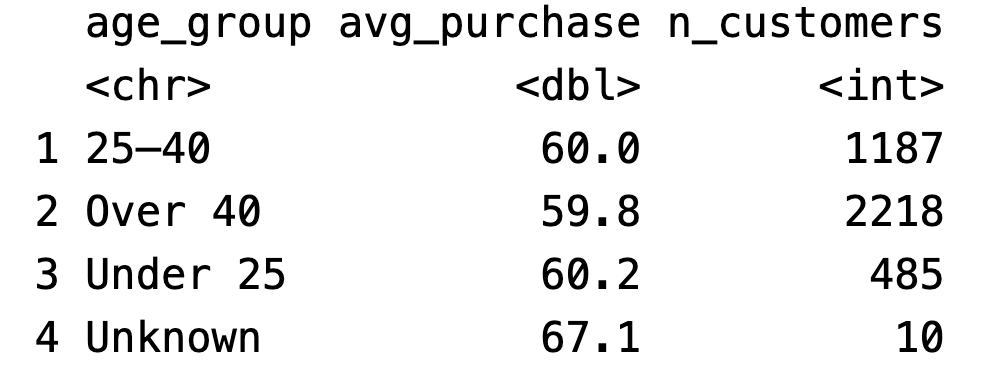
\includegraphics[width=0.6\linewidth,height=\textheight,keepaspectratio]{final-outcome.png}

\end{figure}%

\begin{figure}

\caption{\label{fig-final-plot}Simple bar plot}

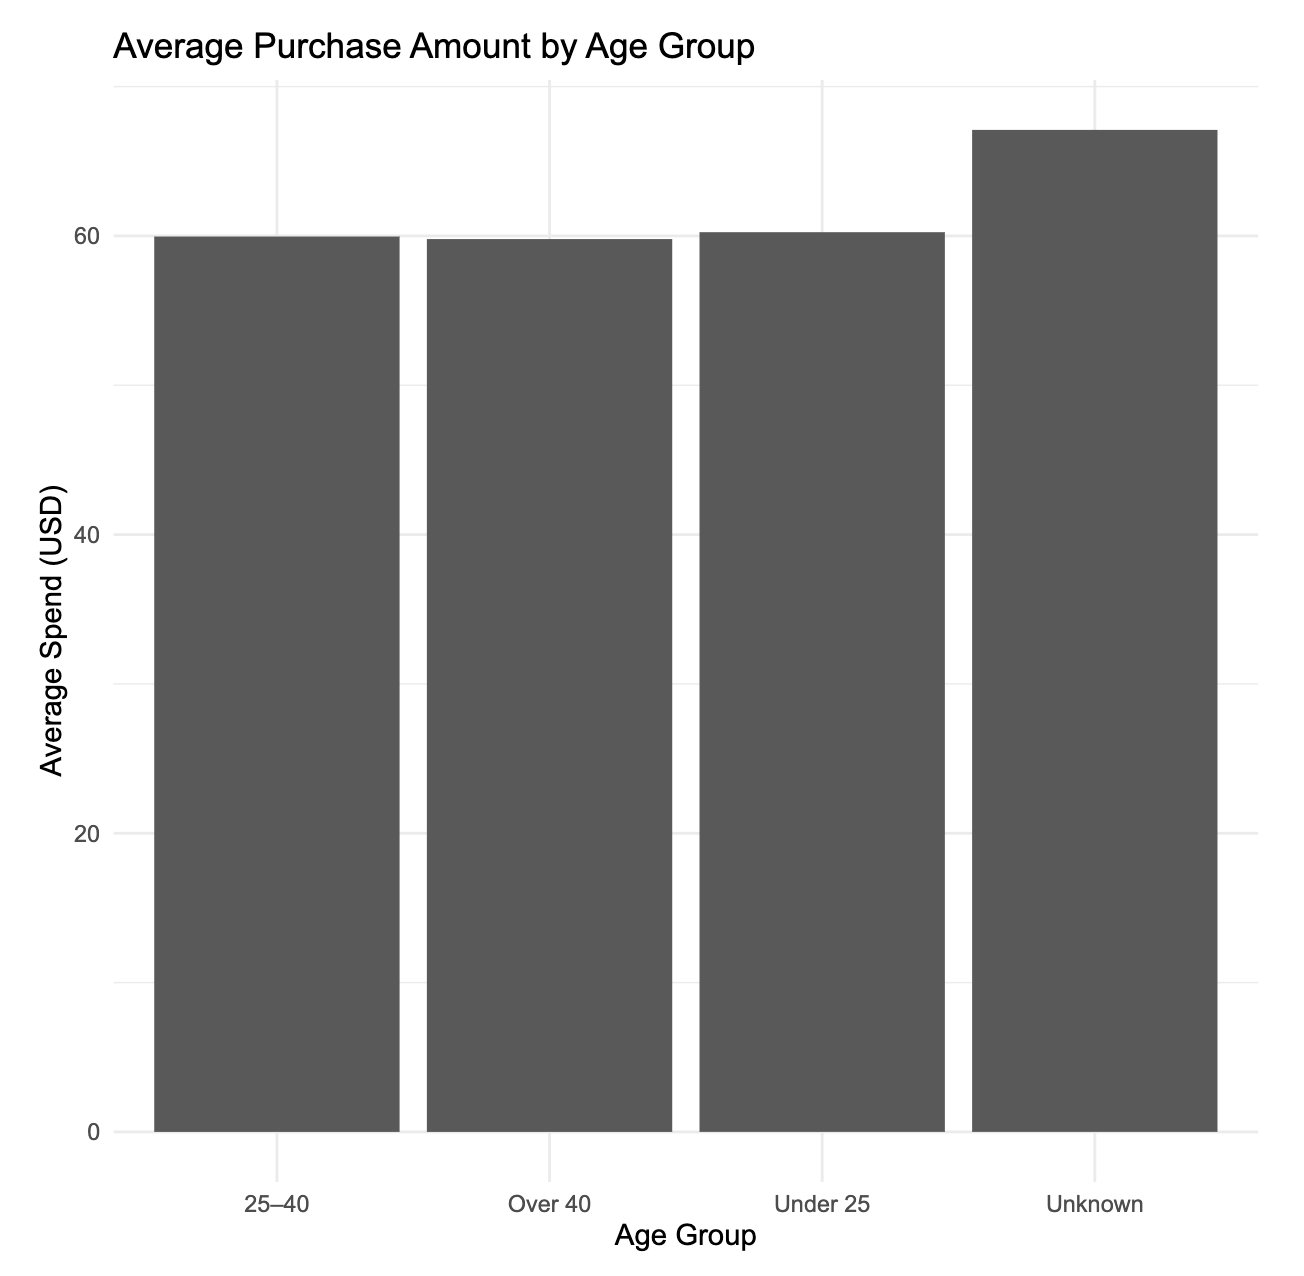
\includegraphics[width=0.6\linewidth,height=\textheight,keepaspectratio]{final-plot.png}

\end{figure}%

\clearpage

\section{References}\label{references}

References marked with an asterisk indicate studies included in the
meta-analysis.

\phantomsection\label{refs}
\begin{CSLReferences}{1}{0}
\bibitem[\citeproctext]{ref-jung2024business}
Jung, D. (2024). Business data understanding. In \emph{The modern
business data analyst: A case study introduction into business data
analytics with CRISP-DM and r} (pp. 49--110). Springer.

\bibitem[\citeproctext]{ref-maskedreference}
Masked Citation. (n.d.). \emph{Masked Title}.

\bibitem[\citeproctext]{ref-Wickham2023R}
Wickham, H., \& Grolemund, G. (2023). \emph{R for data science (2e)}.
\url{https://r4ds.hadley.nz/}

\end{CSLReferences}

\appendix

\section{Affidavit}\label{apx-affidavit}

I hereby affirm that this submitted paper was authored unaided and
solely by me. Additionally, no other sources than those in the reference
list were used. Parts of this paper, including tables and figures, that
have been taken either verbatim or analogously from other works have in
each case been properly cited with regard to their origin and
authorship. This paper either in parts or in its entirety, be it in the
same or similar form, has not been submitted to any other examination
board and has not been published.

I acknowledge that the university may use plagiarism detection software
to check my thesis. I agree to cooperate with any investigation of
suspected plagiarism and to provide any additional information or
evidence requested by the university.

Checklist:

\begin{itemize}
\tightlist
\item[$\boxtimes$]
  The handout contains 3-5 pages of text.
\item[$\boxtimes$]
  The submission contains the Quarto file of the handout.
\item[$\boxtimes$]
  The submission contains the Quarto file of the presentation.
\item[$\boxtimes$]
  The submission contains the HTML file of the handout.
\item[$\boxtimes$]
  The submission contains the HTML file of the presentation.
\item[$\boxtimes$]
  The submission contains the PDF file of the handout.
\item[$\boxtimes$]
  The submission contains the PDF file of the presentation.
\item[$\boxtimes$]
  The title page of the presentation and the handout contain personal
  details (name, email, matriculation number).
\item[$\boxtimes$]
  The handout contains a bibliography, created using BibTeX with an APA
  citation style.
\item[$\boxtimes$]
  Either the handout or the presentation contains R code that proofs the
  expertise in coding.
\item[$\boxtimes$]
  The filled out Affidavit.
\item[$\boxtimes$]
  The link to the presentation and the handout published on GitHub.
\item[$\square$]
  In group work, each student's contribution is clearly defined, and
  individual performance can be assessed using specified sections, page
  numbers, or other objective criteria.
\end{itemize}

{[}Karla Hernández,{]} {[}2025-02-17,{]} {[}Köln, Germany{]}






\end{document}
